\section{A taxonomy of positioning signals}
\label{sec:taxonomy}

Everything tested falls into six classes. The class structure is not
decorative: outcomes are homogeneous \emph{within} class and the two
laws of Section~\ref{sec:laws} explain the pattern \emph{across}
classes.

\begin{description}
\item[A. Conviction and positioning changes.] Counts of costly
  actions: new top-of-book entries (NCB), top-decile holdings growth,
  breadth changes, entry/exit rates. \emph{Where the alpha lives.}
\item[B. Flow and forced selling.] The manager-level implied-flow
  instrument and its stock-level projections: forced-sale supply
  (FSS), flow-driven demand pressure, synthetic short interest.
  \emph{The mechanism engine; prices as a regime-dependent short.}
\item[C. Crowding and ownership states.] Levels: days-of-ADV held,
  ownership share, holder concentration, institutional-ownership
  changes, factor crowding, co-ownership graphs, latent-strategy
  crowding. \emph{Fifteen formulations, zero predictors --- Law 1.}
\item[D. Smart money and universe selection.] Performance-weighted
  votes, skill scores, manager filters. \emph{Zero of nine, with the
  root cause measured (skill persistence 0.25).}
\item[E. Latent structure.] ICA on flow panels, NMF on portfolio
  weights. \emph{Valid identification instruments; modest tradable
  edge, reported as such.}
\item[F. Event-clock and tactical.] Ragged per-name entry, quarter-end
  effects, amendment events, daily stress detection, monitors.
  \emph{The clock studies; one anti-panic rule and one risk
  conditioner survive.}
\end{description}

\subsection{The seventeen-signal catalogue}
\label{sec:catalogue}

Class A--C constructions were evaluated jointly as a pre-registered
catalogue of seventeen signals under the Section~\ref{sec:protocol}
protocol, each with a literature anchor where one exists, each
evaluated raw and residualized with the headline version fixed
ex-ante by the dart-throwing test.
Figure~\ref{fig:ic} shows the information coefficients;
Table~\ref{tab:catalogue} the headline statistics. Three facts
matter. First, the ordering: the only $|t|>2.5$ entry is NCB, and the
runner-up is its sibling (top-decile conviction level). Second, the
replication record: where published numbers exist, ours match ---
breadth change replicates \citet{chs2002} at $+1.65\%$/quarter;
institutional-ownership level and share held are dead after size, as
\citet{gompers2001} would predict once their size exposure is
removed and as \citet{chincarini2020} report; days-of-ADV replicates
its published raw value-weighted point ($+1.46\%$/month) and dies
residualized --- the published effect \emph{is} a size/liquidity
exposure. Third, the confidential-treatment reveal group
(\citet{agarwal2013}) does not replicate on our window
($-0.21\%$/quarter, $t=-0.86$).

Three statistical notes discipline the table. \emph{Multiplicity}:
seventeen signals in two versions are 34 tests; the catalogue-wide
Bonferroni bar at the 5\% level is $t\ge3.2$, and NCB is the only
entry that clears it ($t=3.54$) --- though its promotion rests on the
implementation replications and the hyperparameter surface
(Section~\ref{sec:ncb}), not on any single $t$-statistic.
\emph{Magnitude}: an IC of $0.023$ looks small until the fundamental
law of active management prices it ---
$\mathrm{IR}\approx\mathrm{IC}\sqrt{N}$ with $N\approx1{,}900$ names
per quarter gives $\approx1.0$, which is the Sharpe observed;
cross-sectional breadth, not per-name accuracy, is where 13F
information lives. \emph{Weights}: value-weighted variants in the
module reports use the shares-inferred capitalization panel whose
corrupt tail is documented in Section~\ref{sec:lo}; the
equal-weighted headline numbers involve no weights and are
unaffected, and VW columns should be read as indicative only.

\begin{figure}[t]
\centering
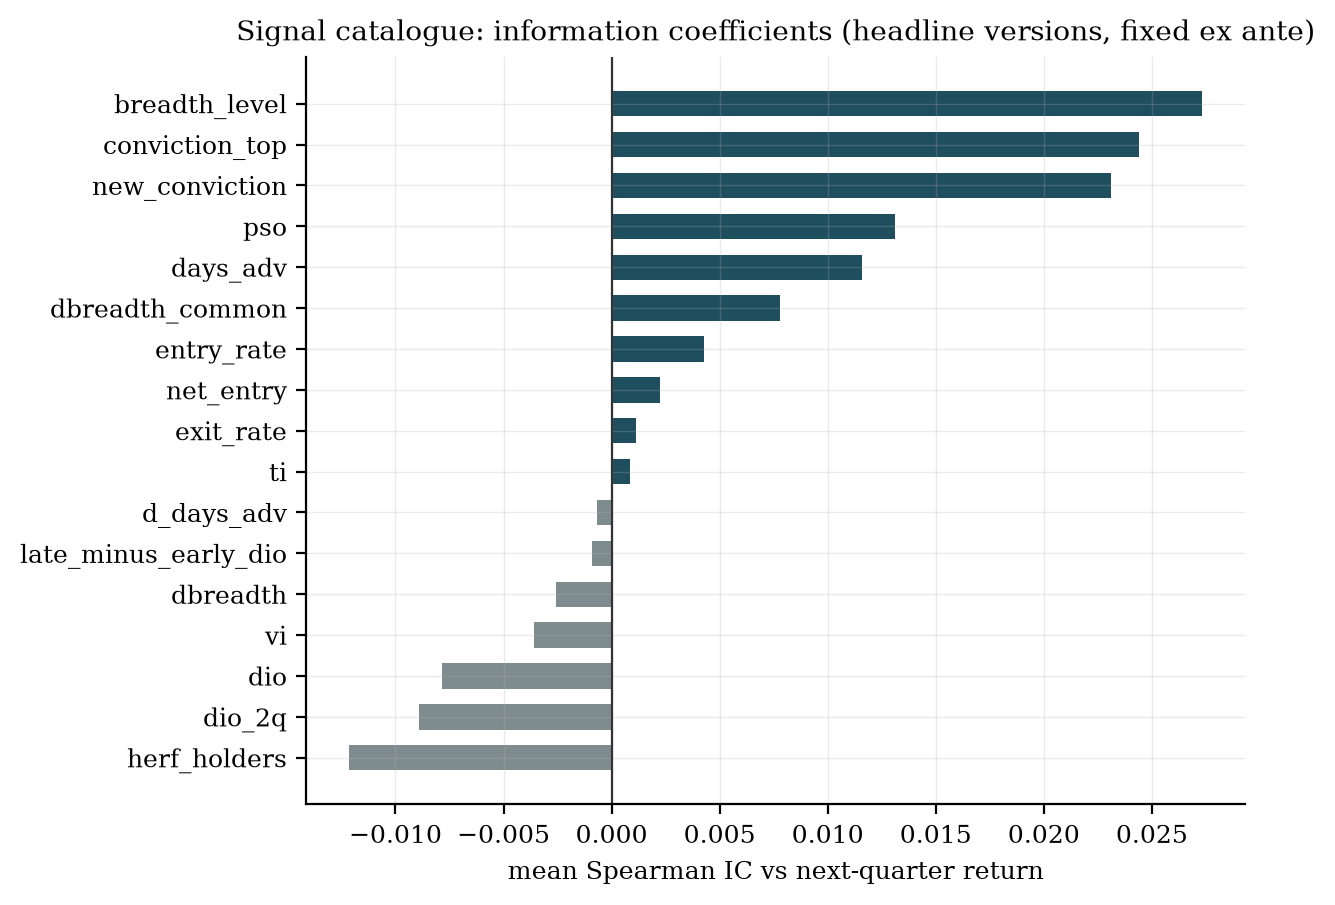
\includegraphics[width=.8\linewidth]{figs/f8_ic_bars.png}
\caption{Mean Spearman information coefficients of the catalogue
(headline versions, fixed ex ante). The conviction family leads;
state variables cluster at zero or negative.}
\label{fig:ic}
\end{figure}

\begin{table}[t]
\centering\footnotesize
\caption{Signal catalogue, headline versions, 49 event quarters.
Spread is the EW Q5$-$Q1 quarterly spread; $t$ is Newey--West;
``resid'' marks signals whose headline is the size/liquidity residual
by the ex-ante placebo rule.}
\label{tab:catalogue}
\begin{tabular}{llrrrrr}
\toprule
signal & version & spread/q & $t$ & Sharpe & IC & mono \\
\midrule
NCB (new\_conviction) & resid & $+0.0218$ & $+3.54$ & $1.08$ & $+0.023$ & $0.58$ \\
conviction\_top & resid & $+0.0223$ & $+2.39$ & $0.65$ & $+0.024$ & $0.58$ \\
breadth\_level & resid & $+0.0193$ & $+1.48$ & $0.36$ & $+0.027$ & $0.55$ \\
late\_minus\_early\_dio & raw & $+0.0068$ & $+1.24$ & $0.34$ & $-0.001$ & $0.53$ \\
entry\_rate & raw & $+0.0134$ & $+1.23$ & $0.36$ & $+0.004$ & $0.57$ \\
dbreadth\_common & raw & $+0.0049$ & $+1.07$ & $0.27$ & $+0.008$ & $0.50$ \\
exit\_rate & raw & $+0.0112$ & $+0.89$ & $0.24$ & $+0.001$ & $0.54$ \\
turnover imbalance & raw & $+0.0031$ & $+0.56$ & $0.13$ & $+0.001$ & $0.51$ \\
value imbalance & raw & $+0.0016$ & $+0.37$ & $0.09$ & $-0.004$ & $0.53$ \\
net\_entry & raw & $+0.0019$ & $+0.33$ & $0.07$ & $+0.002$ & $0.51$ \\
dbreadth & raw & $+0.0022$ & $+0.32$ & $0.06$ & $-0.003$ & $0.53$ \\
$\Delta$days-ADV & resid & $+0.0016$ & $+0.28$ & $0.06$ & $-0.001$ & $0.51$ \\
days-ADV & resid & $-0.0066$ & $-0.41$ & $-0.12$ & $+0.012$ & $0.50$ \\
pct.\ shares held & raw & $-0.0068$ & $-0.74$ & $-0.19$ & $+0.013$ & $0.52$ \\
$\Delta$inst.\ ownership & raw & $-0.0041$ & $-0.76$ & $-0.22$ & $-0.008$ & $0.45$ \\
holder Herfindahl & resid & $-0.0048$ & $-1.09$ & $-0.29$ & $-0.012$ & $0.47$ \\
$\Delta$IO (2q) & raw & $-0.0083$ & $-1.89$ & $-0.46$ & $-0.009$ & $0.48$ \\
\bottomrule
\end{tabular}
\end{table}

\subsection{Replications, stated as such}
\label{sec:replications}

We list the replication record in one place because it calibrates
trust in the new results. \citet{chs2002} breadth: replicated.
\citet{gompers2001} ownership level: the level effect does not
survive size control in the modern sample, consistent with the
mechanism being institutional \emph{flows} into preferred
characteristics rather than the level itself. Days-of-ADV
(\citet{chincarini2020} and related): raw point replicated, removed
by residualization. \citet{agarwal2013} confidential holdings: not
replicated on 2013--2025. \citet{miori2022} position-imbalance
reversal: evaluated in its oracle form and after bias correction
(Section~\ref{sec:tactical}); the adjusted premium is materially
smaller. \citet{coval2007}: the mechanism (redemption-driven selling)
replicates with $t=+20.9$; the expected-flow \emph{forecasting}
construction does not transfer to 13F-implied flows
(Section~\ref{sec:fss}). \citet{kps2019} IPCA and the bootstrap
selection protocol of \citet{oliveira2025} are applied as
methodology, each with its own verdict.
